\chapter{Developer Documentation}
\label{chapter:DevDoc}

\section{Architectural Overview}
\label{sec:Arch}

Figure~\ref{fig:Arch} provides an overview of the system. The clang-plugin
developed produces a database for each translation-unit, which can then be
merged to make all variable declarations available to the frontend, which can
then suggest names for the variables.

The structure of the database can be seen in Figure~\ref{fig:Database}.

%Hack to get the stereo to be aligned next to the line instead of on it.
\newcommand{\stereorelation}[5]{
	#1[#3]{#4}{#5}
	#1[arg1=$\ll$#2$\gg$, pos1=0.5]{#4}{#5}
}

\begin{figure}
	\label{fig:Arch}
	\caption{Overview of Architectural Elements}
	\begin{center}
		\begin{tikzpicture}

			\umlclass[x=0, y=0]{header}{}{}
			\umlclass[x=0, y=-3]{source}{}{}
			\umlclass[x=5, y=-3]{clang}{}{}
			\umlclass[x=5, y=0]{plugin}{}{}
			\umlclass[x=10, y=0]{database}{}{}
			\umlclass[x=10, y=-3]{frontend}{}{}

			\stereorelation{\umlaggreg}
					{includes}{mult1=*, mult2=*}{source}{header}
			\stereorelation{\umluniassoc}
					{compiles}{mult1=1, mult2=*}{clang}{source}
			\stereorelation{\umluniassoc}
					{invokes}{mult1=1, mult2=1}{clang}{plugin}
			\stereorelation{\umluniassoc}
					{produces}{}{plugin}{database}
			\stereorelation{\umluniassoc}
					{loads}{mult1=1, mult2=*}{frontend}{database}

		\end{tikzpicture}
	\end{center}
\end{figure}

\begin{figure}
	\label{fig:Database}
	\caption{Structure of the Database}
	\begin{center}
		\begin{tikzpicture}
			\umlclass[x=0, y=0]{Database}{}{}
			\umlclass[x=5, y=0]{VariableDeclaration}{
				name: string \\
				type: string \\
				location: string
			}{}
			\umlclass[x=5, y=-5]{VariableOccurence}{
				location: string
			}

			\umlcompo[mult1=1, mult2=*]{Database}{VariableDeclaration}
			\umlcompo[mult1=1, mult2=*]{VariableDeclaration}{VariableOccurence}
		\end{tikzpicture}
	\end{center}
\end{figure}

\subsection{Database Format}
\label{sec:dbfmt}
The database produced by the compiler-plugin generates a list of declarations
that are later used for suggesting variables.
The database format is designed such that each translation unit creates its own
database, so that when a project is being built with a build-system that
supports incremental building, wherein a source change only causes the impacted
source file to be recompiled, the database produced for that source file can
then be recombined with the rest, to produced a complete overview of all
variables in the project.

To support renaming of variables, we also need to track the location of any
references to the variables. This is to ensure that after renaming the
variable name at the point of declaration, we also must update every part of the
code that refers to this variable. This can not be achieved by mere textual
pattern-matching, as multiple scopes may have variables of the same name. This
means we have to list all occurences during analysis. When merging the databases
we also need to merge the list of occurences.

\section{Clang-plugin Architecture}

\begin{figure}
	\label{fig:Plugin}
	\caption{Structure of the Clang-plugin}
	\begin{center}
		\begin{tikzpicture}
			\begin{umlpackage}{clang}
				\umlsimpleclass[x=0, y=0]{FrontendPluginRegistry};
				\umlsimpleclass[x=5, y=0]{PluginASTAction};
				\umlsimpleclass[x=0, y=-2]{ASTConsumer};
				\umlsimpleclass[x=5, y=-2, template={Derived}]{RecursiveASTVisitor};
			\end{umlpackage}
			\begin{umlpackage}{dn}
				\umlclass[x=5, y=-7]{Action}{
					std::unique\_ptr$<$Consumer$>$ CreateASTConsumer(...) \\
					bool ParseArgs(...) \\
					ActionType getActionType()
				}{};
				\umlinherit{Action}{PluginASTAction};
				\umlclass[x=0, y=-10]{Consumer}{
					void HandleTranslationUnit(...)}{};
				\umlinherit{Consumer}{ASTConsumer}
				\stereorelation{\umluniassoc}
						{creates}{mult1=1, mult2=1}{Action}{Consumer};
				\umlclass[x=7, y=-10]{Visitor}{
					bool VisitDecl(Decl*) \\
					bool VisitStmt(Stmt*)
				}{};
				\umlinherit{Visitor}{RecursiveASTVisitor};
				\stereorelation{\umluniassoc}
						{invokes}{mult1=1, mult2=1}{Consumer}{Visitor};
				\umlclass[x=0, y=-13]{VariableDeclaration}{
					std::string getLocation(SourceManager\&) \\
					void addOccurence(...)
				}{
					std::string name, type \\
					SourceLocation location \\
					std::vector$<$std::string$>$ occurences
				};
				\stereorelation{\umluniassoc}
						{generates}{mult1=1, mult2=*}{Visitor}{VariableDeclaration};
			\end{umlpackage}
		\end{tikzpicture}
	\end{center}
\end{figure}

The clang-plugin contains all the code needed for traversing the Abstract
Syntax Tree, along with the routines needed for dumping the names that occur in
the codebase to a JSON file. All code in the clang-plugin is defined in
\lstinline|namespace dn|.

The plugin first starts by loading \lstinline|Action| into
\lstinline|clang::FrontEndPluginRegistry|. \lstinline|Action| can then parse the
command-line arguments passed to Clang, so that it can deduce the filename that
was set for storing the output JSON. \lstinline|Action| uses
\lstinline|clang::PluginASTAction::ActionType Action::getActionType()| to inform
Clang that \lstinline|Action| should not inhibit compilation, and should be
invoked after the compilation has been done.

Clang then loads the \lstinline|Consumer| as specifed by
\lstinline|Action::CreateASTConsumer|, which can then proceed with traversing
the Abstract Syntax Tree of the given Translation Unit.

\lstinline|Consumer|'s sole responsibility is to invoke the \lstinline|Visitor|
when invoked by Clang.

\section{Implementation}
\subsection{Merging the Databases}

The database format as described in \fref{sec:dbfmt} was chosen to enable
merging the databases.
As the database is merely a list of Variables, each with a type, name location
and a list of occurences, these can be merged simply.

Given the following variable:
\begin{lstlisting}[mathescape]
{
	"type": TYPE,
	"name": NAME,
	"location": LOCATION,
	"occurences": [ $\ldots$ ]
}
\end{lstlisting}
and databases $database_1, \ldots, database_n$, we can construct the merged
variable as follows:

\begin{lstlisting}[escapeinside={(*}{*)}]
{
	"type": TYPE,
	"name": NAME,
	"location": LOCATION,
	"occurences": [(*
		\[
			\bigcup_{i=1}^{n}{
				\left \{
					\substack{
						v.occurences \mid v \in database_i.variables \\
						\land v.type = TYPE \\
						\land v.name = NAME \\
						\land v.location = LOCATION
					}
				\right \}
			}
		\]
	*)
	]
}
\end{lstlisting}
